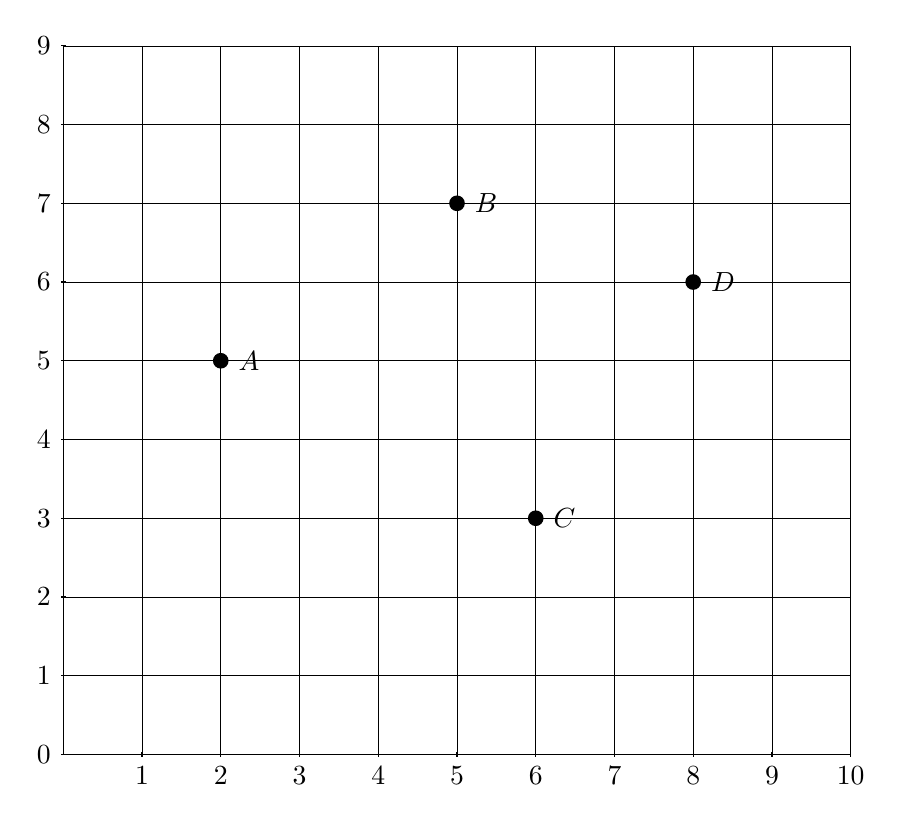
\begin{tikzpicture}
    \draw[step=1cm,very thin]  grid (10,9);
    \foreach \x in {1,2,3,4,5,6,7,8,9,10}
    \draw (\x cm,1pt) -- (\x cm,-1pt) node[anchor=north] {$\x$};
    \foreach \y in {0,1,2,3,4,5,6,7,8,9}
    \draw (1pt,\y cm) -- (-1pt,\y cm) node[anchor=east] {$\y$};
    \node[shape=circle,fill=black, label=right:$A$,scale=0.6] (1) at (2,5){} ;
    \node[shape=circle,fill=black, label=right:$B$,scale=0.6] (1) at (5,7){} ;
    \node[shape=circle,fill=black, label=right:$C$,scale=0.6] (1) at (6,3){} ;
    \node[shape=circle,fill=black, label=right:$D$,scale=0.6] (1) at (8,6){} ;
 \end{tikzpicture}
